%{\it
%Diese Sicht beschreibt den statischen Aufbau des Systems mit Hilfe von
%Modulen, Subsystemen, Schichten und Schnittstellen. 
%Diese Sicht ist hierarchisch, d.h. Module werden in Teilmodule
%zerlegt. Die Zerlegung endet bei Modulen, die ein klar umrissenes
%Arbeitspaket für eine Person darstellen und in einer Kalenderwoche
%implementiert werden können. Die Modulbeschreibung der Blätter dieser
%Hierarchie muss genau genug und ausreichend sein, um das Modul 
%implementieren zu können.
%
%Die Modulsicht wird durch {UML}-Paket- und Klassendiagramme visualisiert.
%
%Die Module werden durch ihre Schnittstellen beschrieben. 
%Die Schnittstelle eines Moduls $M$ ist die Menge aller Annahmen, die
%andere Module über $M$ machen dürfen, bzw.\ jene Annahmen, die $M$
%über seine verwendeten Module macht (bzw. seine Umgebung, wozu auch
%Speicher, Laufzeit etc.\ gehören).
%Konkrete Implementierungen dieser Schnittstellen sind das Geheimnis des Moduls
%und können vom Programmierer festgelegt werden. Sie sollen hier
%dementsprechend nicht beschrieben werden. 
%
%Die Diagramme der Modulsicht sollten die zur Schnittstelle gehörenden Methoden
%enthalten. Die Beschreibung der einzelnen Methoden (im Sinne der Schnittstellenbeschreibung)
%geschieht allerdings per Javadoc im zugehörigen Quelltext. Das bedeutet, dass Ihr
%für alle Eure Module Klassen, Interfaces und Pakete erstellt und sie mit den Methoden der
%Schnittstellen verseht. Natürlich noch ohne Methodenrümpfe bzw.\ mit minimalen Rümpfen.
%Dieses Vorgehen vereinfacht den Schnittstellenentwurf und stellt Konsistenz sicher.
%
%Jeder Schnittstelle liegt ein
%Protokoll zugrunde. Das Protokoll beschreibt die Vor- und
%Nachbedingungen der Schnittstellenelemente. Dazu gehören die erlaubten
%Reihenfolgen, in denen Methoden der Schnittstelle aufgerufen werden
%dürfen, sowie Annahmen über Eingabeparameter und Zusicherungen über
%Ausgabeparameter. Das Protokoll von Modulen wird in der Modulsicht beschrieben.
%Dort, wo es sinnvoll ist, sollte es mit Hilfe von Zustands- oder
%Sequenzdiagrammen spezifiziert werden. Diese sind dann einzusetzen, wenn der
%Text allein kein ausreichendes Verständnis vermittelt (insbesondere
%bei komplexen oder nicht offensichtlichen Zusammenhängen).
%
%Der Bezug zur konzeptionellen Sicht muss klar ersichtlich sein. Im
%Zweifel sollte er explizit erklärt werden. Auch für diese Sicht muss
%die Entstehung anhand der Strategien erläutert werden.
%}

\subsection{Common}
\subsubsection{Entities}
Die \texttt{Common}-Schicht stellt im Paket \texttt{Entities} Klassen bereit, die sowohl von Server als auch Client genutzt werden. Im Mindestfall umfasst dies alle für die Anwendung definierten Datentypen, auf die im nächsten Kapitel näher eingegangen wird.

\begin{figure}[H]
	\centering
	\begin{minipage}[t]{\textwidth}
		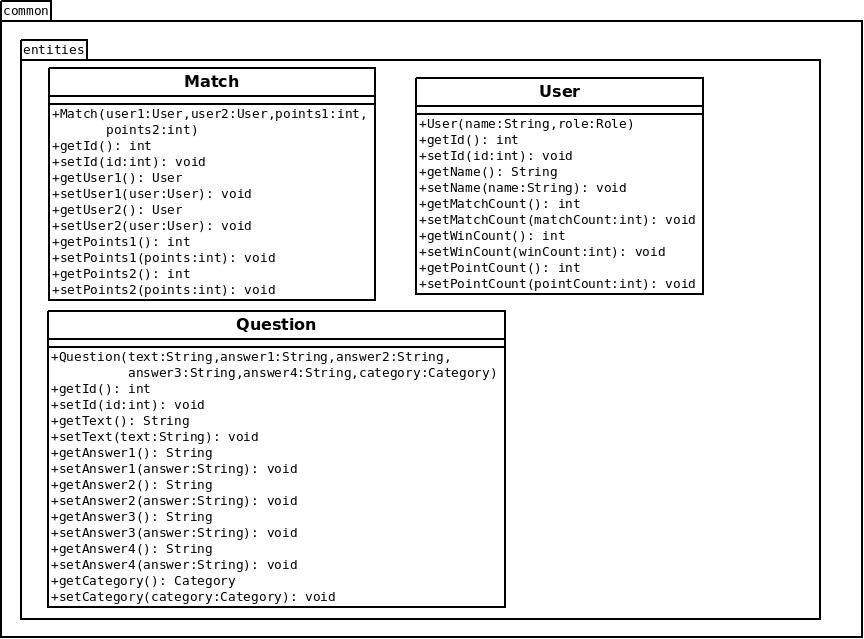
\includegraphics[width=1\textwidth]{Diagramme/entities.jpeg}
		\caption{Entities}
		\label{Entities}
	\end{minipage}
\end{figure}

\subsubsection{Net}
Das \texttt{Net}-Paket enthält eine statische Helferklasse \texttt{NetUtils}, von der Zugangsdaten des Servers abgerufen werden können und in der das Lesen und Schreiben von Sockets implementiert ist. Die Nachrichten, die über die Sockets zwischen Server und Client geschickt werden, sind durch spezielle Klassen definiert, die zur Übertragung in JSON serialisiert und nach der Übertragung deserialisiert werden, um den Informationsaustausch so einfach wie möglich zu machen. Diese Klassen unterteilen sich in \texttt{Requests} und \texttt{Responses}:

\textbf{Requests} werden von einem Client an den Server geschickt, um Daten anzufordern oder mit einem anderen Client zu kommunizieren. 

\textbf{Responses} werden vom Server an einen Client geschickt, um angeforderte Daten zu übertragen oder ihn über etwas zu benachrichtigen. 

Diagramm NetUtils

\subsection{Server}
\subsubsection{Net}
Im \texttt{Net}-Paket ist die Funktionsweise des Servers durch die Klassen \texttt{ServerDirectory} und \texttt{ServerInbox} definiert: Wird er gestartet, wird ein Thread geöffnet, auf dem eine \texttt{ServerDirectory} auf einem Port arbeitet. Die Klasse dient zur Kontaktaufnahme mit den Clients. Für jeden Client wird zudem eine \texttt{ServerInbox} eingerichtet, die - wie der Name schon sagt - als eine Art Postfach für den Server dient und ebenfalls auf einem eigenen Thread läuft. Dort wird für die gesamte Dauer der Verbindung auf Nachrichten des Clients gewartet und anschließend verarbeitet. Ebenfalls ist in der Klasse definiert, wie der Server ggf. auf diese Nachrichten antwortet.

Diagramme ServerDirectory, ServerInbox

\subsubsection{Persistence-Modul}
Die Persistence-Schnittstelle dient zum Zugriff auf die Datenbank und ist wie folgt definiert:

Diagramm IPersistence

\subsection{App-Client}
\subsubsection{Net}
Die \texttt{Client}-Klasse öffnet ein Socket zum Server und implementiert Methoden, um \texttt{Requests} an den Server zu senden. Analog zur \texttt{ServerInbox} wird auch hier ein Thread gestartet, auf dem eine \texttt{ClientInbox} läuft. Diese bearbeitet vom Server empfangene Nachrichten, indem die jeweilige Methode des Game-Moduls aufgerufen wird.

Diagramm ClientInbox

\subsubsection{Game-Modul}
Die Game-Schnittstelle definiert, welche Funktionalität die App bieten muss und beeinflusst dadurch essentiell Spielmechanik und Menüführung:

Diagramm IGame

\subsection{HTML-Client}
Beim HTML-Client beschränkt sich die Kommunikation mit dem Server auf HTTP-Anfragen. Je nachdem, auf welche Adresse zugegriffen wird, werden intern Methoden ausgeführt, um die benötigten Daten darzustellen. Im folgenden sollen deshalb den möglichen Pfaden Methoden zugeordnet werden.

\begin{table}[h]
    \begin{tabular}{|l|l|l|l|}
    \hline Pfad & Methode & Request & Parameter\\ 
    \hline /login & ~ & POST & name, password\\ 
    	\hline
    \end{tabular}
\end{table}